\documentclass[aspectratio=169]{beamer}
\setbeamertemplate{navigation symbols}{}
\usepackage{color,amsmath,comment, subfigure}
\usepackage{booktabs}
\usepackage{url}

%\setbeameroption{show notes}

%%%%%%%%%%%%%%%%%%%%%%%%%%
\title[]{Lecture 5: Degree distributions and power laws}
\author[]{Matthew J. Salganik}
\institute[]{Sociology 204: Social Networks, Spring 2021\\Princeton University}
\date[]{
1/2: Scale-free networks

\vfill

\begin{flushleft}
\vspace{0.7in}

\includegraphics[width=0.05\textwidth]{figures/cc.png}
\end{flushleft}
}

\begin{document}
%%%%%%%%%%%%%%%%%%%%%%%%%%%
\frame{\titlepage}
%%%%%%%%%%%%%%%%%%%%%%%%%%%
\begin{comment}
\begin{frame}

SWBAT:
\begin{enumerate}
\item recognize networks that are scale-free and networks that are not scale-free
\item explain the data generating process for scale-free networks
\item explain the abstract similarity between Watts and Strogatz and Barabasi and Albert 
\end{enumerate}

\end{frame}
\end{comment}
%%%%%%%%%%%%%%%%%%%%%%%%
\begin{frame}

Review:
\begin{itemize}
\item simple model (ring lattice + rewiring) predicts that many networks will be ``small-world'' networks 
\pause
\item three real networks (movie actors, power grid, and worm brain) have high clustering coefficient (relative to Erdos-Renyi random graph) and similar characteristic path length to Erdos-Renyi random graph
\pause
\item abstract model helps us understand many types of networks
\pause
\item these network structural properties are important for dynamics happening on the network (e.g., disease spread)
\end{itemize}

\note{Now we are going to see the same trick again.  Abstract model, new properties of networks, important for dynamics.  

For some this will be too mathematical, for some not mathematical enough.  I don't expect you to derive any of this or prove any of this.  That would be for a different class.}

\end{frame}
%%%%%%%%%%%%%%%%%%%%%%%%%
\begin{frame}

\begin{figure}
  \centering
   \subfigure{
   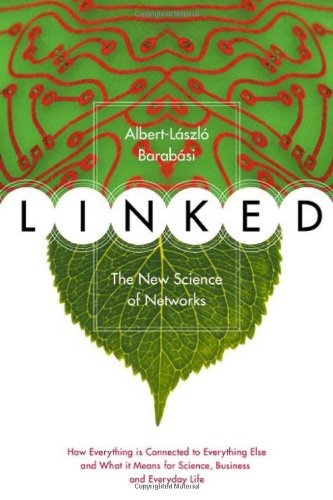
\includegraphics[width=0.35\textwidth]{figures/barabasi_linked_2002_cover}}
  \hspace{0.1\textwidth}
    \subfigure{
   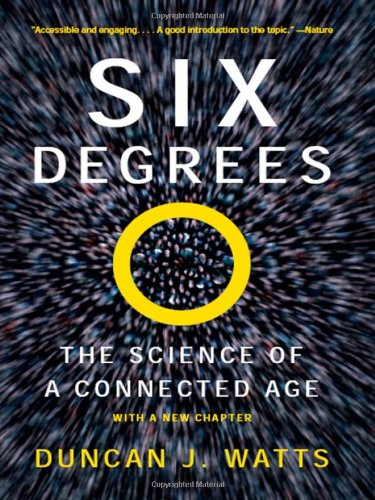
\includegraphics[width=0.35\textwidth]{figures/watts_six_2003_cover}}
    \hspace{0.1\textwidth}
\end{figure}

\note{
Talk about parallels in the work between Barabasi and Watts. Timing of papers and books in the transformation of the study of networks around 2000.
}

\end{frame}
%%%%%%%%%%%%%%%%%%%%%%%%%%%%
\begin{frame}

\begin{itemize}
\item degree: number of connections that a node has to other nodes (not related to degrees of separation)
\item degree distribution: distribution of degrees
\end{itemize}

\note{Last class the main quantities of interest were characteristic path length and clustering coefficient.  This time degree and degree distribution.  

What is a degree distribution? Think about how many friends you have on Facebook?  If everyone in the class 

Also, Watts and Strogatz were not interested in this because they were thinking about social networks.  Barabasi was interested in the world wide web so degree was a very natural quantity of interest.  Sometimes it is having a different background or interest that enables you to ask a more interesting questions.}

\end{frame}
%%%%%%%%%%%%%%%%%%%%%%%%%%%%
\begin{frame}

\setcounter{subfigure}{0}% Reset subfigure counter
\begin{figure}
  \centering
     \subfigure[Normal]{
     \label{fig:normal} % Label for first subfigure
     \includegraphics[width=0.40\textwidth]{figures_book/4_1}}
  \hspace{0in}
  \subfigure[Power law]{
     \label{fig:6_4} % Label for second subfigure
     \includegraphics[width=0.40\textwidth]{figures_book/4_2}}
     \label{fig:degree_dist} % Label for entire figure
\end{figure}

\pause
\vfill
\onslide<2-3>{Is the distribution of heights more similar to normal or scale-free?} \onslide<3>{normal}\\
\onslide<4-5>{Is the distribution of wealth more similar to normal or scale-free?} \onslide<5>{scale-free}\\


\note{
Is the distribution of heights more similar to normal or scale-free? [vote]\\
Is the distribution of wealth more similar to normal or scale-free? [vote]\\
For example, city size and income are power law distributed, height and weight are normal\\
}

\end{frame}
%%%%%%%%%%%%%%%%%%%%%%%%%%%%
\begin{frame}

\setcounter{subfigure}{0}% Reset subfigure counter
\begin{figure}
  \centering
  \subfigure[Power law]{
     \label{fig:6_4} % Label for second subfigure
     \includegraphics[width=0.45\textwidth]{figures_book/4_2}}
  \subfigure[log-log Power law]{
     \label{fig:6_4} % Label for second subfigure
     \includegraphics[width=0.45\textwidth]{figures_book/4_3}}
\end{figure}

\note{
logging pulls in extreme values

Power laws are straight lines on log-log plot, log pulls in big values\\
Don't show but if asked\\
$p(k) \propto \frac{1}{k^n}$\\
$log p(k) \propto log(\frac{1}{k^n})$\\
$log p(k) \propto log(1) - log(k^n)$\\
$log p(k) \propto - n log(k)$\\
}

\end{frame}
%%%%%%%%%%%%%%%%%%%%%%%%%%
\begin{frame}

\setcounter{subfigure}{0}% Reset subfigure counter
\begin{figure}
  \centering
  \subfigure[Power law]{
     \label{fig:6_4} % Label for second subfigure
     \includegraphics[width=0.25\textwidth]{figures_book/4_2}}
  \subfigure[log-log Power law]{
     \label{fig:6_4} % Label for second subfigure
     \includegraphics[width=0.25\textwidth]{figures_book/4_3}}
\end{figure}

\pause

$p(k) \propto \frac{1}{k^n}$\\ \pause
$log p(k) \propto log(\frac{1}{k^n})$\\ \pause
$log p(k) \propto log(1) - log(k^n)$\\ \pause
$log p(k) \propto - n log(k)$\\ 

\note{
logging pulls in extreme values

Power laws are straight lines on log-log plot, log pulls in big values\\
Don't show but if asked\\
$p(k) \propto \frac{1}{k^n}$\\
$log p(k) \propto log(\frac{1}{k^n})$\\
$log p(k) \propto log(1) - log(k^n)$\\
$log p(k) \propto - n log(k)$\\
}

\end{frame}
%%%%%%%%%%%%%%%%%%%%%%%%%%\begin{frame}
\begin{frame}

It turns out that many degree distributions follow a power law distribution (which Barabasi calls ``scale-free'')\\
$p(k) \sim \frac{1}{k^{\gamma}}$

\begin{center}
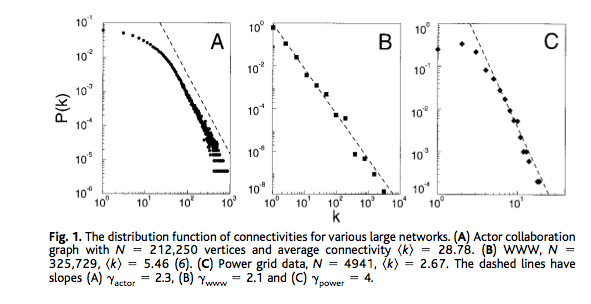
\includegraphics[width = 0.95\textwidth]{figures/barabasi_emergence_1999_fig1}
\end{center}

\end{frame}
%%%%%%%%%%%%%%%%%%%%%%%%%%%
\begin{frame}

\onslide<1-2>{Does $\beta$ model produce power law degree distribution?} \onslide<2>{No}

\begin{center}
\includegraphics[width = 0.8\textwidth]{figures_book/3_6}
\end{center}

\note{
Explain why this graph is not power law
}


\end{frame}
%%%%%%%%%%%%%%%%%%%%%%%%%%%
\begin{frame}

Barabasi and Albert propose a very simple model that generates networks with power law degree distributions

\begin{itemize}
\item growth (new nodes enter the system)
\item preferential attachment (more likely to connect to high degree nodes)
\end{itemize}

\note{
If models are poetry, this model is there poetry.
}

\end{frame}
%%%%%%%%%%%%%%%%%%%
\begin{frame}

Demo

\url{http://www.netlogoweb.org/launch\#http://ccl.northwestern.edu/netlogo/models/models/Sample\%20Models/Networks/Preferential\%20Attachment.nlogo}

\note{
Look at this picture.  Is there anything that you notice about it?

Mental checklist of networks.
- degree distribution
- average path length (hard to eyeball)
- clustering coefficient

Is this clustering coefficient high or low?
This is different from many real social networks.  Many real social networks have lots of triangles in part for reasons you will learn about next class.

The point is to remind you about clustering coefficient and encourage you to think about connections between models
}

\end{frame}
%%%%%%%%%%%%%%%%%%%%%%%%%%
\begin{frame}


\end{frame}
%%%%%%%%%%%%%%%%%%%%%%%%%%

\end{document}
